\documentclass[11pt]{article}
\usepackage[margin=0.8in]{geometry}\usepackage{amsmath,amssymb,graphicx,booktabs,tabularx,hyperref}
\setlength{\parindent}{0pt}\setlength{\parskip}{7pt}
\begin{document}
{\LARGE Target information in retained relations}\par
2026-10-30. Derived diagnostic and synthetic correctness controls.

For a consistent system $Ax+bk+c=0$ over a prime field, the target $k$ is uniquely determined exactly when $b$ is outside the column space of $A$. Equivalently,
\[\operatorname{rank}[A\ b]-\operatorname{rank}A=1.\]
Consistency is tested separately by $\operatorname{rank}[A\ b\ c]=\operatorname{rank}[A\ b]$. An inconsistent system is never reported as determining a valid target.

\textbf{Derivation.} Subtract any two solutions. If $b\notin\operatorname{col}A$, a nonzero difference in $k$ would express $b$ as a linear combination of columns of $A$, a contradiction. Conversely, if $b=Av$, every solution extends to $(x-tv,k+t)$ for every field element $t$, so $k$ is not unique. Existence is why consistency is checked first.

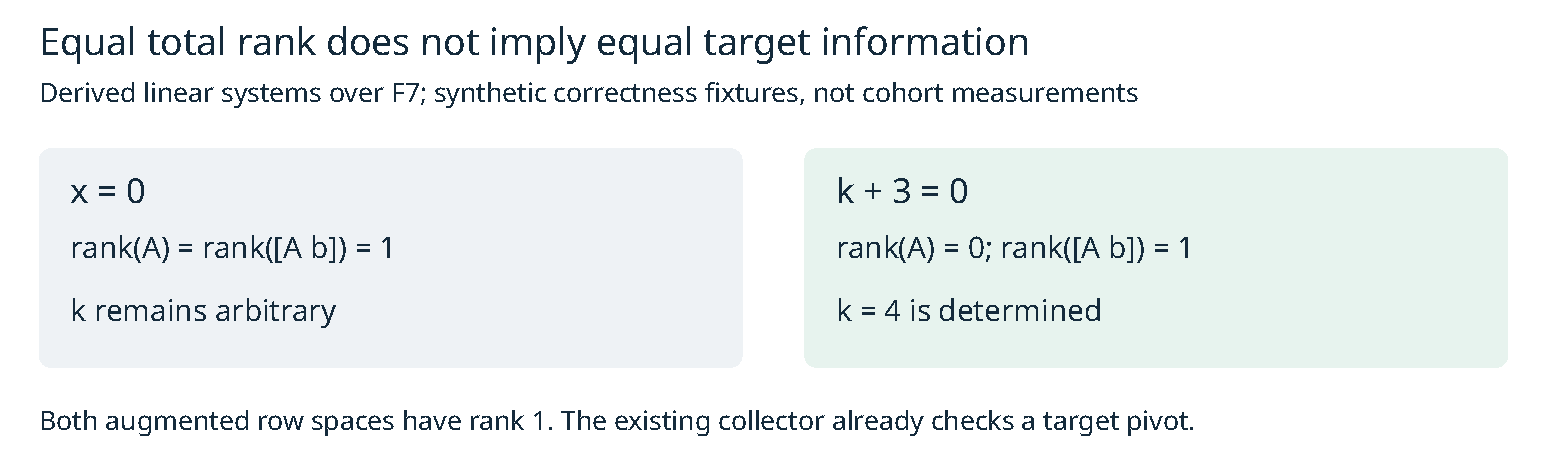
\includegraphics[width=\textwidth]{information.pdf}

\textbf{Source observation.} The existing GraphSolver in \texttt{native\_solver.rs} already checks a target-column pivot after an independent admission (lines 500--516 at the recorded source). This packet does not introduce a new stopping rule. It adds an offline diagnostic to separate nuisance rank from target information.

\newpage
{\Large Implementation and review boundary}\par
The diagnostic reuses the existing prime-field residual basis three times, projecting to nuisance columns, nuisance plus target, and all columns. Rows have a fixed width and composite moduli are rejected by the existing basis constructor. It does not alter collection, elimination order, enrollment, or original results.

\textbf{Controls.} Six native unit tests passed: equal total rank with different information; nuisance-rank growth; inconsistency; row reordering/scaling and empty systems; wrong-domain/shape rejection; and direct enumeration of solution sets for fixed small algebraic fixtures. These are software correctness checks, not scientific samples or a cohort experiment. Native fixture output retains all five example matrices.

\textbf{Cost boundary.} Three basis computations incur additional work and mutate the kernel's thread-local operation counters. The diagnostic must run outside a measured producer. No time, memory advantage or end-to-end ratio is claimed. Replaying a fixed relation stream cannot establish a changed collector policy's future collection cost.

\textbf{Remaining evidence.} Independent source review is pending. This packet does not reconstruct per-relation information histories from aggregate historical rank counters. A subsequent policy comparison needs an actual retained relation stream, or prospectively reviewed instrumentation and a separate frozen evaluation. Existing 1,260-target obligations remain unchanged.

\textbf{Artifacts.} \texttt{result.json} contains formulas, scope and exact fixture results; \texttt{information.svg} is editable; source, validation logs and the source manifest accompany the report. No scalar search or new curve experiment was performed.
\end{document}